\documentclass[10pt,a4paper]{article}
\usepackage[utf8]{inputenc}
\usepackage[T1]{fontenc,url}
\usepackage{multicol}
%\usepackage{parskip}
\usepackage{lmodern}
\usepackage{microtype}
\usepackage{verbatim}
\usepackage{amsmath, amssymb}
\usepackage{tikz}
\usepackage{physics}
\usepackage{mathtools}
\usepackage{algorithm}
\usepackage{algpseudocode}
\usepackage{listings}
\usepackage{enumerate}
\usepackage{graphicx}
\usepackage{float}
\usepackage{hyperref}
\usepackage{siunitx}
\usepackage{framed}
\usepackage{multirow}
\usepackage{pdfpages}
\usepackage[a4paper, margin=0.2cm]{geometry}
\renewcommand{\baselinestretch}{1}
\setlength\parindent{0pt}

\renewcommand{\exp}{e^}
\newcommand{\half}{\frac{1}{2}}
\renewcommand{\b}{\textbf}
\renewcommand{\u}{\underline}
\renewcommand{\i}{\textit}
\newcommand{\gr}{\colorbox{green}}
\newcommand{\yl}{\colorbox{yellow}}

\setlength{\columnsep}{0.4cm}
\setlength{\columnseprule}{0.06cm}
\setlength{\FrameSep}{0.2cm}

%\setlength{\columnseprule}{1pt}

\begin{document}
\begin{multicols}{2}


\section*{Sammendrag}
\subsection*{Viktige formler}
\begin{framed}
\b{Termodynamikkens 1. Lov:} $\Delta U = Q + W$ \\ \\
\b{Termodynamisk identitet:} $\dd U = T\dd S - P\dd V + \mu \dd N$
\\ \\
\b{Termodyn. identitet for G:} $\dd G = -S \dd T + V\dd P + \mu \dd N$
\\ \\
(Hint for termodynamiske identiteter: Stryk ledd for å få definisjoner.)
\end{framed}
\subsection*{Ordbok}
\begin{itemize}
	\item kvasistatisk - Uniformt trykk og temperatur. 
	\item Adiabatisk - Ingen varmeoverføring (i.e. raske endringer).
	\item Isotermisk - Konstant temperatur (i.e. sakte endringer).
\end{itemize}

\subsection*{Regneregler}
\begin{align*}
	&\ln{n^x} = x\ln{n} \quad\quad \ln(xy) = \ln{x}+\ln{y} \\
	&\ln{1+x} \approx x \quad\quad x (\rightarrow 0)
\end{align*}


\section{Energi i termofysikk}
\subsection*{Ideell gass}
\begin{framed}
Ideell gas lov. Ideell gass holder for lav tetthet, ingen interaksjon mellom partiklene, og bare (3) translatoriske frihetsgrader.
\begin{align*}
	PV = NkT = nRT
\end{align*}
der $N$ er antallet molekyler, $n$ er antall mol av molekyler, og $R$ er en gasskonstant.
\end{framed}

\subsection*{Ekvipartisjonsprinsippet og frihetsgrader}
\begin{framed}
\b{Kvadratiske frihetsgrader:} Kvadratiske funksjoner av posisjon eller hastighet som kan lagre energi. 3 translatoriske, 3 rotasjonsgrader(inntrer ved lav temperatur, kan være færre, avhengig av symertri), 3 vibrasjonsgrader(inntrer ved høy temperatur, kan være færre).
\\ \\
\b{Ekvipartisjonsprinsippet} forteller oss den termiske energien til en gass fra temperaturen og frihetsgradene:
\begin{align*}
	U_{termisk} = Nf\frac{1}{2}kT
\end{align*}
\end{framed}


\subsection*{Varme og arbeid}
\begin{oframed}
\b{Varme} - $Q$: Spontan overføring av energi til et annet grunnet temperaturforskjell. \b{Leding}, \b{Konveksjon}, eller \b{Stråling}.

\b{Arbeid} - $W = \int\limits_{V_1}^{V_2}P(V)\dd{V}$.\\
Arbeid kommer somregel i form av kompresjon av et volum:
\begin{itemize}
	\item \b{Kvasistatisk} kompresjon: Sakte nok til at gassen rekker å oppnå likevekt med omgivelsene. Uniform trykk og temperatur i gassen.
	\item \b{Isoterm} kompresjon: $ W = NkT\ln{\frac{V_1}{V_2}}$ \\
	Sakte, konstant $T$ med omgivelsene.
	\item \b{Adiabatisk} kompresjon: $ V^\gamma P = const. \quad \gamma = f(f+2)$ \\
	Rask, ingen tid til varmeoverføring $Q=0$.
\end{itemize}
\end{oframed}

\subsection*{Varmekapasitet}
\begin{oframed}
Defineres som varme(energi) som trengs for å øke noe én grad, $C = Q/\Delta T$. Ved konstant volum(ingen arbeid på gassen, $W = 0)$ får vi
\begin{align*}
	C_V = \qty(\frac{\Delta U}{\Delta T})_V = \qty(\pdv{U}{T})_V
\end{align*}
Konstant trykk gir derimot
\begin{align*}
	C_P = \qty(\frac{\Delta U - (-P\Delta V)}{\Delta T})_P = \qty(\pdv{U}{T})_P + P\qty(\pdv{V}{T})_P
\end{align*}
\\

\b{Latent varme:} Ved faseoverganger øker ikke temperaturen ved tilførsel av energi. Da er varmekapasiteten per def uendelig: $C = Q/\Delta T = Q/0 = \infty$. Energien som kreves for å fullføre faseoverangen kalles den latente varmen $L = Q/m$, og er varmen per masse som kreves.
\\

\b{Entalpi:} Energien til et system, pluss energien som trengs for å sette systemet i omgivelsene (dytte bort atmosfæren). $H = U + PV$.
\end{oframed}



\section{Termodynamikkens 2. lov}

\subsection*{Kombinatorikk}
\begin{framed}
\u{\b{Fundamentalt stat-mek prinsipp:}}\\
I et \b{isolert} system i \b{likevekt} er alle tilgjengelige mikrotilstander like sannsynlige.

\begin{itemize}
\item \b{Mikrotilstand:} Unik konfigurasjon av systemet, der partikkeltilstanden til alle pariklene er spesifisert.
\item \b{Makrotilstand:} En system-tilstand med en bestemt makroskopisk egenskap (speisifik temperatur, energi...)
\item \b{Multiplisitet, $\Omega$:} Antallet mikroilstanden for en gitt makrotilstand.
\item \b{Sannsynligheten} for at et system er i en makrotilstand $s_i$ er direkte proporsjonalt med multiplisiteten til tilstanden: $P(s_i) = \frac{\Omega(s_i)}{\sum\Omega(s_i)}$.
\end{itemize}
\end{framed}


\subsection*{To-tilstands problem}
\begin{framed}
For et $N$-partikkel-system med $n$ partikler i en tilstand og $N-n$ i den andre tilstanden, er multiplisiteten til tilstanden
\begin{align*}
	\Omega(N,n) = \begin{pmatrix} N\\ n \end{pmatrix}
	= \frac{N!}{n!\cdot (N-n)!}
\end{align*}
Dette tilsvarer både mulige måter å plukke $n$ elementer fra $N$, eller mulige måter å sortere $n$ og $N-n$ elementer seg imellom.
\end{framed}


\subsection*{Paramagnetisme}
\begin{framed}
$N$ magneter som kan peke opp eller ned. \b{Mikrotilstandene} er unike konfigurasjoner av opp/ned. \b{Makrotilstandene} er totalt anntall opp/ned. Multiplisiteten er $\Omega(N_{\uparrow}) = \begin{pmatrix}N\\N_\uparrow\end{pmatrix}$
\end{framed}
\newpage


\subsection*{Einstein-krystall}
\begin{framed}
Fast stroff der hvert atom sees på som 3 harmoniske oscilatorer med diskret energinivåer. $N$ atomer, og $q$ "energienheter", som kan fordeles på oscilatorene. Multiplisiteten er da gitt som
\begin{align*}
	\Omega = \begin{pmatrix} q+N-1\\ q \end{pmatrix}
	= \frac{(q+N-1)!}{q!(N-1)!} \approx \qty(\frac{eq}{N})^N
\end{align*}
Der siste ledd er en tilnærming ved høytemperatur-grensen $q >> N$ med Stirlings Approksimasjon.
\end{framed}

\subsection*{Vekselvirkende system}
\begin{framed}
System av to Einsten-krystaller som kan utveksle energienheter. Total multiplisitet $\Omega_{tot} = \Omega_a + \Omega_b$.
\end{framed}


\b{Stirling Aproksimasjon:} \yl{$N! \approx N^N e^{-N}\sqrt{2\pi N} \approx N^N e^{-N}$}


\subsection*{Enatomig ideell gass med N partikler}
\begin{framed}
Utledning viser at multiplisiteten til en slik gass er $\Omega(U,V,N) \approx f(N)V^N U^{3N/2}$ der $f(N)=\frac{1}{N!}\frac{1}{h^{3N}}\frac{\pi^{3N/2}}{(3N/2)!}(2m)^{3N/2}$.
\end{framed}


\subsection*{Entropi}
\begin{framed}
Et isolert system i likevekt har en overveldende sannsynlighet til å konvergere mot en makrotilstand med høyest mulig multiplisitet. Etter lang tid vil systemet nesten alltid finnes rundt den høyeste multiplistiteten.\\
Entropien til et system har en tendens til å øke.
\b{Entropi:} $S = k\ln{\Omega}$

\b{Regneregler:} Fordi multiplisitet er multiplikativt, $\Omega_{tot} = \Omega_a\Omega_b$, legges entropiendringer sammen; $\Delta S_{tot} = \Delta S_a + \Delta S_b$.

\subsubsection*{Entropiøkning fra blanding}
Blander vi to forskjellige gasser av $N$ partikler, øker entropien med
\begin{align*}
	\Delta S_{tot} = \Delta S_a + \Delta S_b = 2Nk\ln{2}
\end{align*}
\end{framed}




\section{Interaksjon og implikasjoner}
\subsection*{Oppsummering - Interaksjoner}
\resizebox{0.5\textwidth}{!}
{
	\begin{tabular}{||c  c  c  c||}
		\hline
		\b{Type} &  \b{Utvekslet} &  \b{Bestemmende}   & \multirow{2}{1.5cm}{\b{Formel}} \\
		\b{Interaksjon}  &  \b{Kvantitet}  &  \b{Variabel} & \\
		\hline
		Termisk  &  Energi  &  Temperatur  &   $\frac{1}{T} = \qty({\pdv{S}{U}})_{V,N}$ \\
		\hline
		Mekanisk  &  Volum  &  Trykk  &  $\frac{P}{V} = \qty(\pdv{S}{V})_{U,V}$ \\
		\hline
		Diffusivt  &  Partikler  &  Kjemisk pot.  &  $\frac{\mu}{T} = - \qty(\pdv{S}{N})_{U,V}$\\
		\hline
	\end{tabular}
}


\subsection*{Temperatur}
\begin{framed}
Sett to forskjellige materialer i kontakt. Ved termisk likevekt kan vi observere at $\pdv{S_A}{U_A} = \pdv{S_B}{U_B}$. Altså, tilførsel av litt energi ville gitt like mye entropi til begge materialene. Observerer også at materialer med lavere energi har brattere S mot U grafer, slik at en tilførsel av energi gir høy entropiøkning, og de vil tendere til å ta imot energi. Dette kjenner vi igjen som lav temperatur. Vi kan dedusere relasjonen
\begin{align*}
	\frac{1}{T} = \qty(\pdv{S}{U})_{N,V}
\end{align*}
\end{framed}


\subsection*{Fremgangsmåte for å finne varmekapasitet for et system}
\begin{framed}
\begin{enumerate}
	\item Bruke kvantemekanikk og/eller kombinatorikk til å finne et uttrykk for multiplisiteten som funksjon av $U$, $V$, $N$ og andre variable.
	\item Finne entropien, $S=k\ln{\Omega}$
	\item Derivere entropi mhp. energi for å finne temperatur som funksjon av energi, og evt. andre variable.
	\item Deriver $U(T)$ med hensyn på $T$ for å finne varmekapasitet (med andre variable holdt konstant).
\end{enumerate}
\end{framed}


\subsection*{Paramagnetisme (Varmekapasitet)}


\subsection*{Termodynamikkens 3. Lov}
\begin{framed}
\begin{align*}
	T \rightarrow 0 \quad \Rightarrow \quad C_V \rightarrow 0 
\end{align*}
\end{framed}


\subsection*{Entropi og varmekapasitet}
\begin{framed}
Definisjonen av temperatur gir eventuelt en definisjon av entropi som
\begin{align*}
	\dd S = \frac{\dd U}{T} = \frac{Q}{U} = \frac{C_V \dd T}{T}
\end{align*}
gitt \b{ingen arbeid og kvasistatisk}. Dette gir oss mulighet til å regne ut entropi (i teorien helt fra T=0):
\begin{align*}
	\Delta S = \int\limits_{T_i}^{T_f}\frac{C_V}{T}\dd T
\end{align*}
\end{framed}


\subsection*{Mekanisk likevekt og trykk}
\begin{framed}
Mekanisk likevekt skjer ved konstant trykk. Dette skjer ved $\pdv{S_A}{V_A} = \pdv{S_B}{V_B}$. 

Vi kan definere trykk som
\begin{align*}
	P = T\qty(\pdv{S}{V})_{U,N}
\end{align*}
\end{framed}


\subsection*{Diffusiv likevekt}
\begin{framed}
Diffusiv likevekt skjer ved konstant kjemisk potensial, $\mu$. Dette skjer ved $\pdv{S_a}{N_a} = \pdv{S_b}{N_b}$.

Vi kan definere kjemisk potensial som
\begin{align*}
	\mu = -T\qty(\pdv{S}{N})
\end{align*}
\end{framed}



\section{Varmemaskin og kjøleskap}
\subsection*{Varmemaskin}
\begin{framed}
En varmemaskin absorberer en varme $Q_h$ fra et \b{varmt reservoar} ved temperatur $T_h$, og konverterer en andel av energien til arbeid, $W$. Rest-varmen $Q_c$ dumpes i et \b{kaldt reservoar} ved temperatur $\mathbf{T_c}$. Reservoarene er store nok til at temperaturen ikke endres.
\begin{figure}[H]
\centering
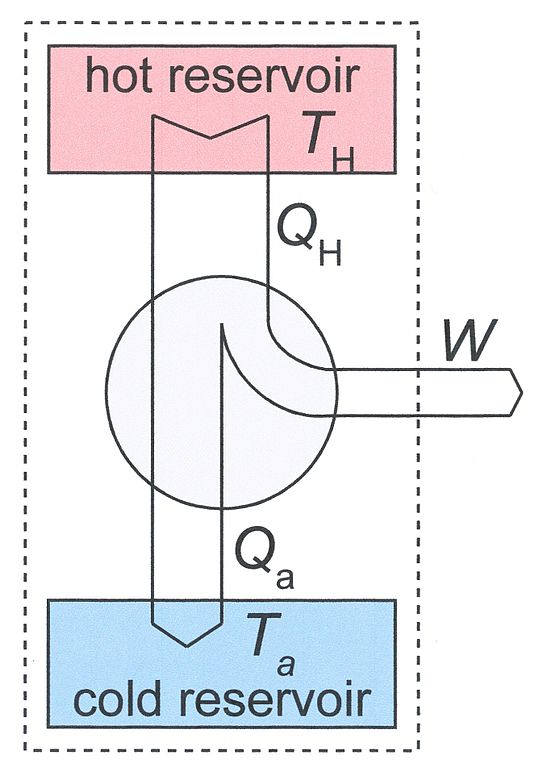
\includegraphics{{figures/heat_engine.jpg}}
\end{figure}

\b{Effektiviteten} defineres som andelen av varmen $Q_a$ som blir konvertert til arbeid:
\begin{align*}
	e = \frac{utbytte}{kostnad} = \frac{W}{Q_h} = \frac{Q_h - Q_c}{Q_h} = 1 - \frac{Q_c}{Q_h}
\end{align*}
\b{Maksimal Effektivitet:} Entropien som ankommer det kalde reservoaret $S_c = Q_c/T_c$, må være minst like stor som entropien som forlater det varme reservoaret $S_h = Q_h/T_h$:
\begin{align*}
	\frac{Q_c}{T_c} \geq \frac{Q_h}{T_h} \quad \Rightarrow \quad \frac{Q_C}{Q_h} \geq \frac{T_c}{T_h} \quad \Rightarrow \quad e \leq 1 - \frac{T_c}{T_h}
\end{align*}
\end{framed}


\subsection*{Carnot Syklusen}
\begin{framed}
Carnot-syklusen representerer den optimalt effektive varmemaskinen.

\begin{enumerate}
	\item Isotermisk Ekspansjon: Temperatur holdes infititesimalt under $Q_h$ (for minimal entropiøkning) ved å sakte øke volumet.\\
	\item Adiabatisk ekspansjon: Øker volumet til temperaturen har sunket til $~T_c$.
	\item Isoterm kompresjon: Temperaturen holdes infititesimalt over $Q_c$ (for minimal entropiøkning) ved å sakte senke volumet.\\
	\item Adiabatisk kompresjon: Senker volumet til temperaturen har økt til $~T_h$.
\end{enumerate}
\end{framed}


\begin{figure}[H]
\centering
	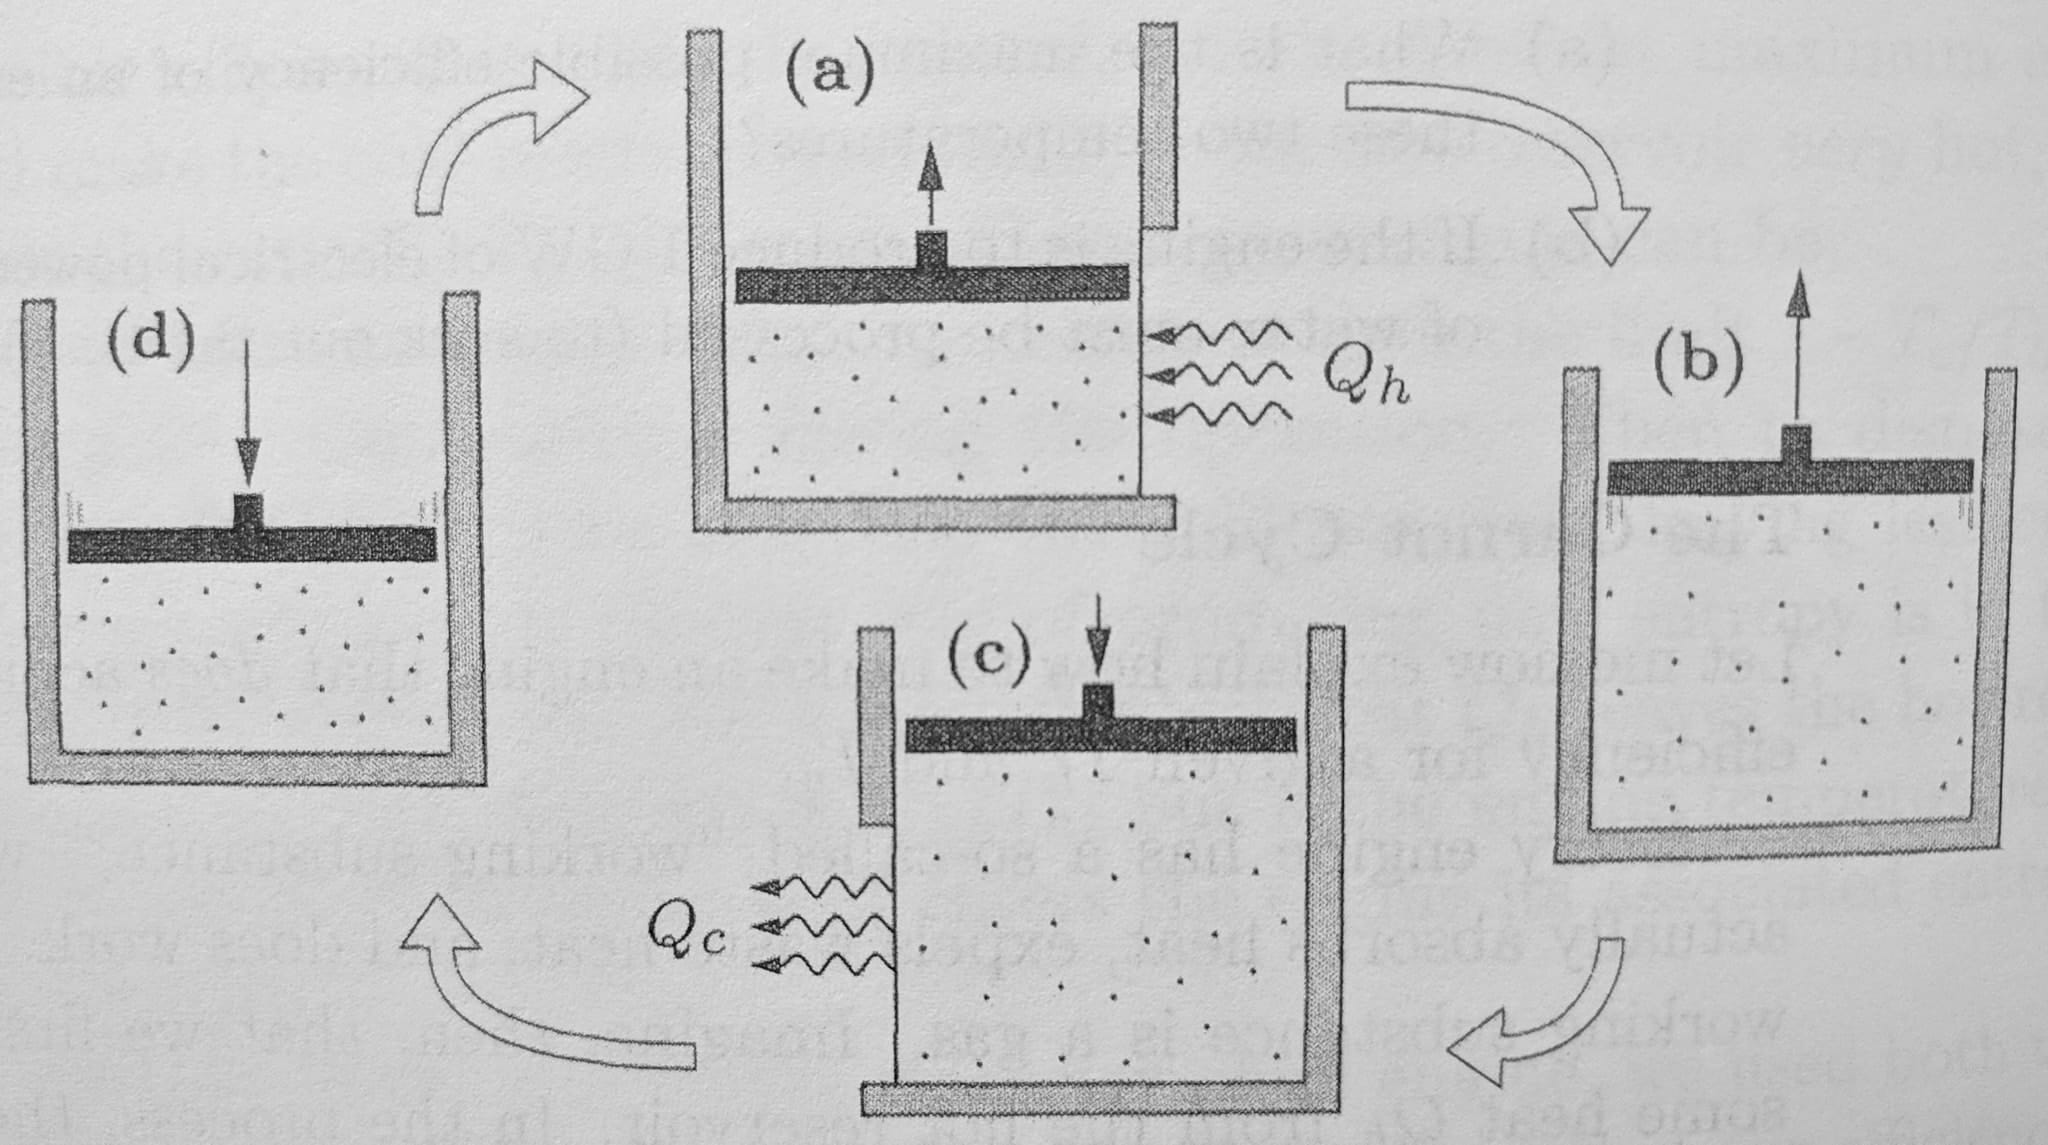
\includegraphics[width=0.4\textwidth]{figures/carnot_cycle2.jpg}
\end{figure}

\begin{figure}[H]
\centering
	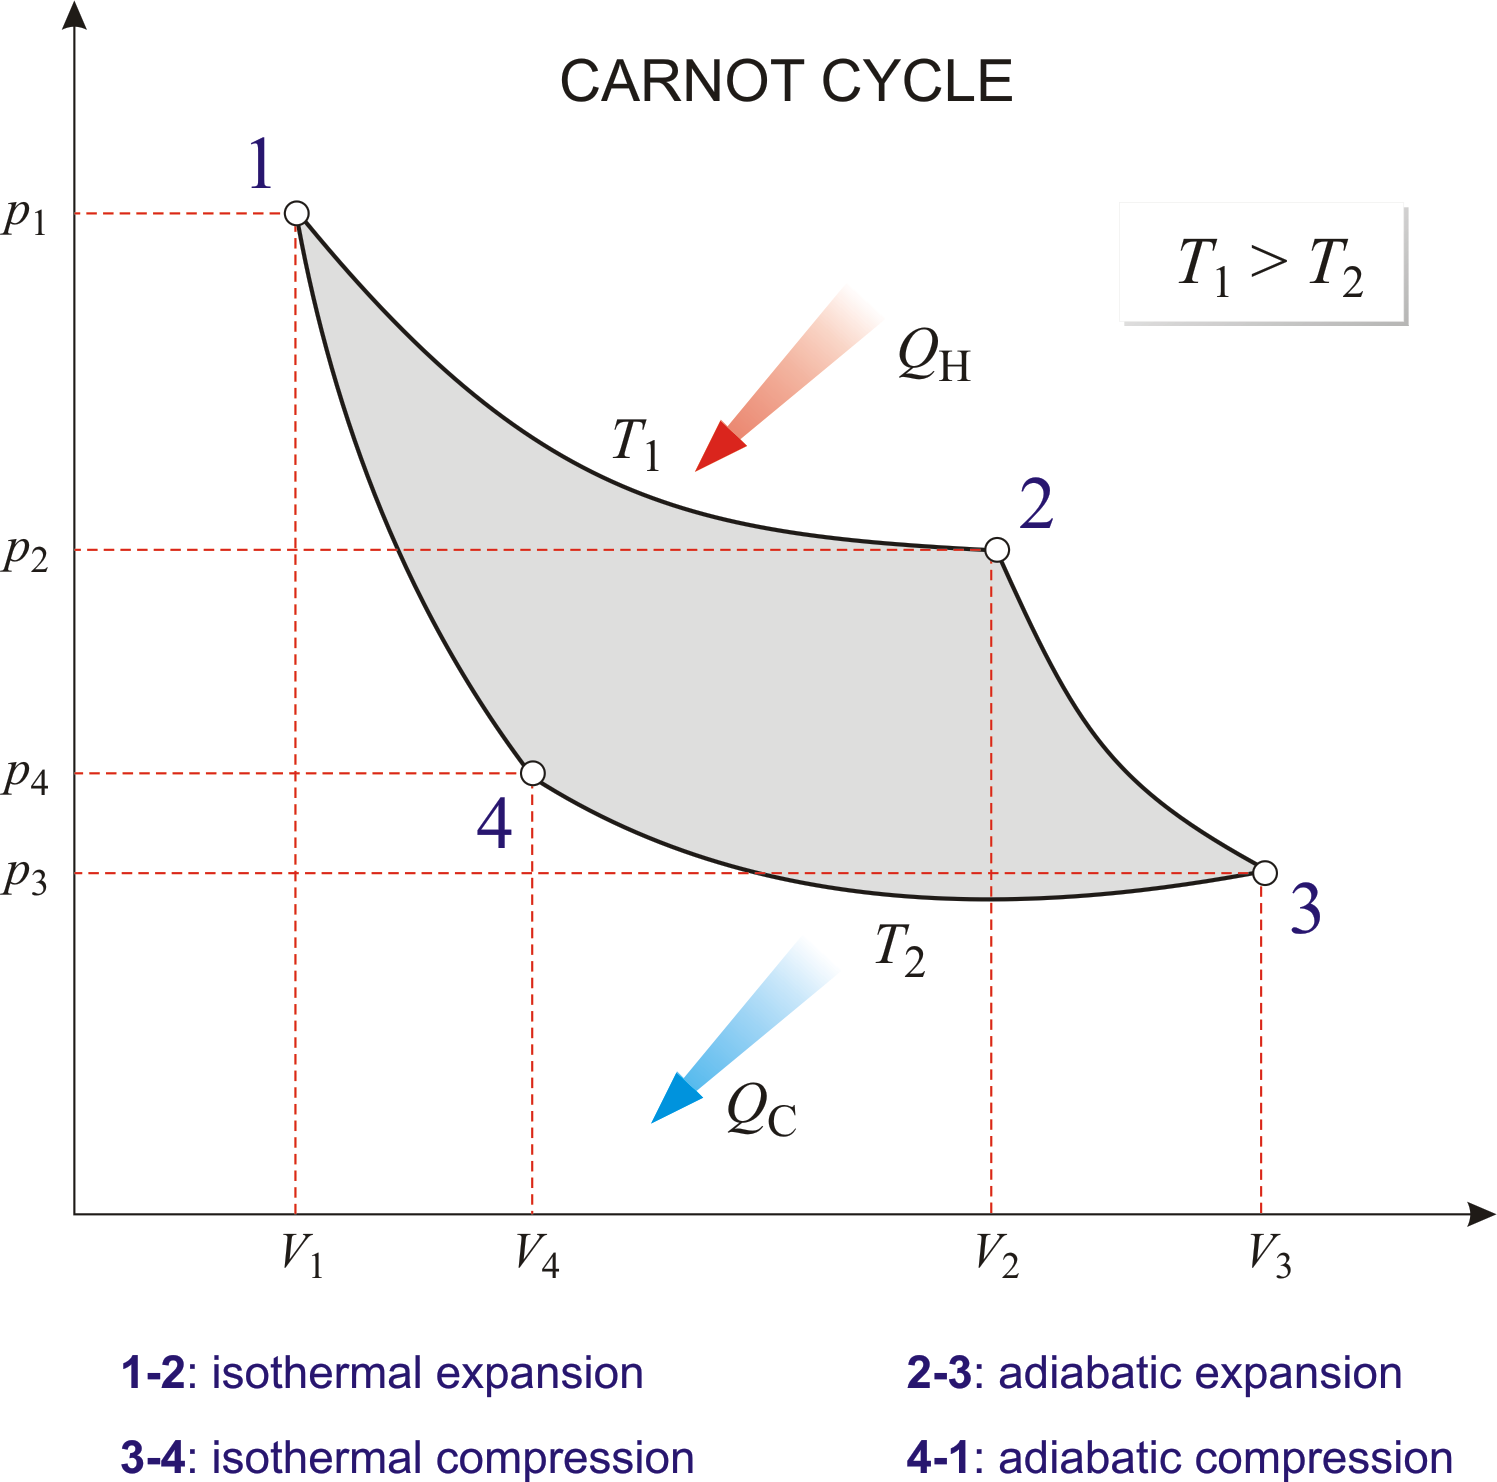
\includegraphics[width=0.3\textwidth]{figures/carnot_cycle.png}
\end{figure}

\subsection*{Kjøleskap}
\begin{framed}
Et kjøleskap er en varmemaskin i revers. Den bruker eksternt arbeid til å overføre varme fra det kalde til det varme reservoaret.

Vi introduserer kjøleskapets effektivitet:
\begin{align*}
	COP = \frac{utbytte}{kostnad} = \frac{Q_c}{W} = \frac{Q_c}{Q_h-Q_c} = \frac{1}{Q_h/Q_c - 1}
\end{align*}
Tilsvarende entropilogikken for varmemaskinen får vi \b{maks effektivitet:}
\begin{align*}
	COP \leq \frac{1}{T_h/T_c - 1}
\end{align*}
\end{framed}




\section{Fri energi og kjemisk termodyniamikk}
\subsection*{Fri energi som tilgjengelig arbeid}
\begin{framed}
\gr{\u{\b{Entalpi:}}} Energien til systemet pluss energien som trengt for å lage plass til det (dytte vekk omgivelsene). \\
\b{Def:} \colorbox{yellow}{$H = U + PV$} \\
\b{Termodyn. id.:} \colorbox{yellow}{$\dd H = T\dd S + V\dd P + \mu \dd N$}
\\ \\ \\
\gr{\u{\b{Helmholtz frie energi:}}} Energien til systemet, minus (varme)energien systemet kan få gratis fra omgivelsenes temperatur. (alt. def i kap. 6) \\
\b{Def:} \colorbox{yellow}{$F = U - TS$} \\
\b{Termodyn. id.:} \colorbox{yellow}{$\dd F = -S\dd T - P\dd V + \mu \dd N$}
\\ \\ \\
\gr{\u{\b{Gibbs frie energi:}}} Kombinasjon av bidragene fra $H$ og $F$. \\
\b{Def:} \colorbox{yellow}{$G = U - TS + PV$}.\\
\b{Termodyn. id.:} \colorbox{yellow}{$\dd G = -S\dd T + V\dd P + \mu \dd N$}
\end{framed}
\i{Hint:} Sett enkelte av variablene konstante for å utlede definisjoner, i.e.:
$ S = -\qty{\pdv{G}{T}}_{P,N}$
\\
\newpage


\begin{framed}
\b{Utvidet Termodynamikkens 2. Lov:}
	\begin{itemize}
		\item Ved konstant energi har $S$ en tendens til å øke.
		\item Ved konstant temperatur og volum har $F$ en tendens til å synke.
		\item Ved konstant temperatur og trykk har $G$ en tendens til å synke.
	\end{itemize}
\end{framed}

\begin{framed}
\b{Ekstensive størrelser}(dobles ved dobbelt volum)\\ $V$, $N$, $S$, $U$, $H$, $F$, $G$, $masse$.
\\ \\
\b{Intensive størrelser}(uendret ved volumendring)\\ $T$, $P$, $\mu$, $tetthet$.
\end{framed}




\section{Boltzmann Statistikk}
Ser på systemer(f.eks. et atom) i kontakt med et stort reservoar. Antar at det er liten sannsynlighet for at samme partikler ønsker å oppta samme tilstand (lav tetthet).
\\ \\
\b{Degenerasjon:} Hvis flere tilstander $s_i$ svarer til samme energinivå, sier vi at systemet er degenerert. Vi må da huske at sannsynligheten for å finne systemet ved det gitte energinivået er summen av sannsynlighetene for alle tilstandene med det energinivået (degenerasjonsgraden).


\subsection*{Boltzmann faktoren}
\begin{framed}
\begin{align*}
	\exp{-E(s)/kT}
\end{align*}
Representerer en ikke-normalisert sannsynlighet for å finne systemet i en tilstand $s$. Kan brukes til å finne forholdet mellom sannsynlighetene for to tilstander:
\begin{align*}
	\frac{P(s_2)}{P(s_1)} = \frac{\Omega_R(s_2)}{\Omega_R(s_1)} = \frac{\exp{S_R(s_2)/k}}{\exp{S_R(s_1)/k}}= \exp{[S_R(s_2) - S_R(s_1)]/k} \\
	= \exp{-[E(s_2) - E(s_1)]/kT} = \frac{\exp{-E(s_2)/kT}}{\exp{-E(s_1)/kT}}
\end{align*}
der vi har brukt den termodynamiske identiteten med $\dd N = \dd V \approx 0$ for å få at $S_R(s_2) - S_R(s_1) = -1/T[E(s_2) - E(s_1)]$
\end{framed}


\subsection*{Partisjonsfunksjonen}
\begin{framed}
Partisjonsfunksjonen er essensielt (den inverse) normaliseringsfaktoren til Boltzmann faktoren, slik at vi kan få den faktiske sannsynligheten til en tilstand:
\begin{align*}
	P(s) = \frac{1}{Z}\exp{-E(s)/kT}
\end{align*}

Ettersom summen over alle sannsynligheter er $\sum\limits_s P(s) = 1$, blir partisjonsfunksjonen summen over alle Boltzmann faktorene til systemet:
\begin{align*}
	Z = \sum\limits_s \exp{-E(s)/kT}
\end{align*}
\end{framed}

\subsection*{Forventningsverdier/Gjennomsnitt}
\begin{framed}
Gjennomsnitsverdien til en egenskap ved systemet (i.e. energi), er gitt ved
\begin{align*}
	\bar{X} = \sum\limits_s X(s) P(s) = \frac{1}{Z} \sum\limits_s X(s)\exp{-E(s)/kT}
\end{align*}

\i{Hint:} Gjennomsnitt er additative. For eksempel er den totale energien til et system gjennomsnittsenergien ganget med antallet partikler: $U = N\bar{E}$
\end{framed}

\subsection*{Partisjonsfunksjonen og fri energi}
Alternativ definisjon av Helmholtz frie energi.
\begin{align*}
	F = -kT\ln{Z} \quad \quad Z = \exp{-F/kT}
\end{align*}


\subsection*{Partisjonsfunksjonen for sammensatte systemer}
\begin{framed}
I utgangspunktet er partisjonsfunksjonen multiplikativ:
\begin{align*}
	Z_{tot} = Z_1Z_2...Z_N \quad \text{(Distinguishable, non-interacting)}
\end{align*}
men dersom partiklene er uadskillbare, kan vi bytte om partiklene uten forskjell, og vi teller samme tilstander to ganger. Generelt får vi
\begin{align*}
	Z_{tot} = \frac{1}{N!}Z_1...Z_N \quad \text{(Indistinguishable, non-interacting)}
\end{align*}
\end{framed}




\section{Kvantestatistikk}
Når tettheten av partikler blir høy, er sannsynligheten for at to partikler ønsker å oppta samme tilstand betydelig. Da bryter antagelsene i Boltzmann statistikken sammen, og vi benytter kvantestatistikk.


\subsection*{Gibbs faktoren og den store partisjonsfunksjonen}
\begin{framed}
Vi utvider Boltzmann statistikk ved å nå tillate utveksling av partikler mellom reservoaret og systemet (diffusiv likevekt). Vi tar da med faktoren $\mu N$ fra den termodynamiske identiteten, som gir sannsynligheten
\begin{align*}
	P(s) = \frac{1}{\mathcal{Z}}\exp{-[E(s) - \mu N(s)]/kT}
\end{align*}

\begin{align*}
	\mathcal{Z} = \sum\limits_s \exp{-[E(s) - \mu N(s)]/kT}
\end{align*}
der $\mathcal{Z}$ kalles \b{Den store partisjonsfunksjonen}, og tilsvarer partisjonsfunksjonen for kvantesystemer. (Eksponent-funksjonen kalles \b{Gibbs-funksjonen})
\end{framed}


\subsection*{Bosoner og fermioner}
\begin{framed}
Når to partikler ønsker å oppta samme tilstand er det to alternativer, avehengig av hva slags partikler det er.
\begin{itemize}
	\item \b{Fermioner} KAN IKKE oppta samme tilstand, og vil "fylle opp" de mulige tilstandene. Vi får da ofte en "fermi-kule" av de opptatte (laveste) energinivåene. 
	\item \b{Bosoner} KAN oppta samme tilstand, i ubegrenset kvantitet.
\end{itemize}
\end{framed}
\newpage


\subsubsection*{Den kvantemekaniske grensen}
\begin{framed}
Vi introduserer "kvantelengden", som er en typisk størrelse på bølgefunksjonen (en faktor $\pi$ fra de Broglie bølgelengden), og "kvantevolumet":
\begin{align*}
	l_Q = \frac{h}{\sqrt{2\pi mkT}}, \quad v_Q = l_Q^3
\end{align*}
Forholdet mellom antallet tilgjengelige tilstander (bestemmes av energi) og partikkeltettheten bestemmer om gassen må behandles med kvantestatistikk:
\begin{align*}
	\frac{V}{N} &\gg v_Q \quad \text{(normal gass)} \\
	\frac{V}{N} &\approx v_Q \quad \text{(quantum gass)}
\end{align*}
Ved \b{lav energi} eller \b{høy tetthet} får vi altså en kvantegass.
\end{framed}


\subsection*{Fordelingsfunksjonen}
Vi ser på en enkelt partikkel-tilstand, som har en energi $\epsilon$ per partikkel som er i tilstanden. Sannsynligheten for å finne  tilstand med $n$ partikler i blir
\begin{align*}
	P(n) = \frac{1}{\mathcal{Z}} \exp{-n(\epsilon-\mu)/kT}
\end{align*}

\subsubsection*{Okkupasjon av tilstand, Fermioner, Fermi-Dirac}
For \b{fermioner} kan antallet bare være 0 eller 1, slik at den store partisjonsfunksjonen blir
\begin{align*}
	\mathcal{Z} = 1 + \exp{-(\epsilon-\mu)/kT} \quad \text{(Fermioner)}
\end{align*}

Vi introduserer \b{sannsynligheten for at en tilstand er okkupert}, eller \b{okkupansen} til en tilstand:
\begin{align*}
	\bar{n} = \sum\limits_n n P(n) = 0P(0) + 1P(1) = \frac{\exp{-[\epsilon - \mu]/kT}}{1 + \exp{-[\epsilon - \mu]/kT}}
\end{align*}
Vi kaller denne fordelingen for \b{Fermi-Dirac fordelingen}:
\begin{align*}
	\bar{n}_{FD}(\epsilon) = \frac{1}{\exp{[\epsilon - \mu]/kT} + 1}
\end{align*}
Vi ser at tilstander med høy energi (iforholdtil $\mu$) har en tendens til å være tomme, mens lav-energi tilstander har en tendens til å være okkupert.
I figured under ser vi okkupans-sannsynlighet for forskjellige temperaturer. Den skarpe overgangen skjer ved $\epsilon=\mu$.
\begin{figure}[H]
\centering
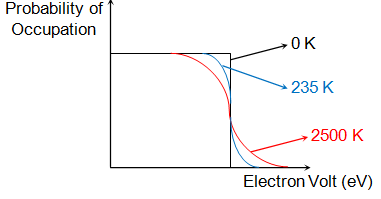
\includegraphics[width=0.3\textwidth]{{figures/fermi_dirac.png}}
\end{figure}

\subsection*{Degenererte Fermi-gasser}
\u{Note:} "Degenerert" har i denne sammenheng ingen relasjon til tidligere bruk av ordet, og betyr at det er en brå overgang mellom okkuperte og ikke-okkuperte energi-tilstander, grunnet veldig lave temperaturer.

\subsubsection*{Temperatur 0K}
Vi ser på en degenerert fermi-gass i en boks av størrelse $L^3 = V$. \\
Ved $T=0$ får vi den skarpe overgangen vi ser i figuren over. Alle tilstandene opp til \b{fermienergien} $\epsilon_F$ vil være okkupert.\\
Energien kommer fra bevegelsesmengde i hver av de 3 frihetsgradene. Denne energien er gitt av bølgefunksjonene i kvantiserte energinivåer:
\begin{align*}
	\epsilon_F = \frac{|\vec{p}|^2}{2m} = \frac{h^2}{8mL^2}(n_x^2 + n_y^2 + n_z^2) = \frac{h^2}{8mL^2}n^2
\end{align*}
Vi kan se på denne energien som et åttendedels kuleskall med radius $n$ (fjerdedels av en sirkel i 2 dim.). Antallet partikler vil da tilsvaret volumet av denne, ganger to, for de to spin-tilstandene. Vi kan da skrive fermienergien som en funksjon av partikkeltettheten:
\begin{align*}
	\epsilon_F = \frac{h^2}{8m}\qty(\frac{3N}{\pi V})^{2/3}
\end{align*}
Den totale energien til gassen blir
\begin{align*}
	U = \int\int\int \epsilon(\vec{n}) \dd n_x \dd n_y \dd n_z = ... = \frac{3}{5}N\epsilon_F
\end{align*}


\subsubsection*{Varmekapasitet, Temperaturer litt over 0}
Ved å la temperaturen gå litt over 0 kan vi regne ut varmekapasiteten:
\begin{align*}
	U = \frac{3}{5}N\epsilon_F + \frac{\pi^2}{4}\frac{N(kT)^2}{\epsilon_F} \quad\quad
	C_V = \qty(\pdv{U}{T})_V = \frac{\pi^2Nk^2T}{2\epsilon_F}
\end{align*}


\subsection*{Tilstandstettheten}
Tilstandstettheten representerer antallet states per per energi ved en gitt energi. Altså tettheten av tilgjengelige tilstander.
\begin{align*}
	D(\epsilon) = \frac{\pi(8m)^{3/2}}{2h^3}V\sqrt{\epsilon} = \frac{3N}{2\epsilon_F^{3/2}}\sqrt{\epsilon}
\end{align*}
Ved \b{temperatur 0} vil totalt antall partikler tilsvare integralet av tilstandstettheten fra 0 til fermienergien. Den totale energien finner vi ved å vekte alle tilstandene med sin energi:
\begin{align*}
	N = \int\limits_0^{\epsilon_F} D(\epsilon) \dd \epsilon \quad\quad
	U = \int\limits_0^{\epsilon_F} \epsilon D(\epsilon) \dd \epsilon \quad\quad (T=0)
\end{align*}
Ved \b{temperatur forskjellig fra 0} vil tilstandene kunne fylle energier over fermi-energien, og alle tilstander under fermi-energien trenger ikke være fylt. Vi må vi også vekte tilstandstettheten med sannsynligheten for at tilstanden er opptatt $\bar{n}_{FD}$ (bare gang inn denne i integralene over, og la dem gå til $\infty$).\\
Vi kan også introdusere tilstandstettheten per $n$, $D(n)$, som bare blir arealet av kuleskallet ganget med de to mulige spinn-tilstandene: $D(n)=2\cdot \frac{1}{8}4\pi n^2 = \pi n^2$, eller i 2 dim: $D(n) = 2\cdot \frac{1}{4}2\pi n = \pi n$.

Vi har også relasjonen \yl{$D(n)\dd n = D(\epsilon)\dd \epsilon$}

\subsection*{Maxwell-relasjonene}
\begin{align*}
	\pdv[2]{U}{S}{V} = \qty(\pdv{T}{V})_S - \qty(\pdv{P}{S})_V \\
	\pdv[2]{H}{S}{P} = \qty(\pdv{V}{S})_P + \qty(\pdv{T}{P})_S \\
	-\pdv[2]{F}{T}{V} = \qty(\pdv{P}{T})_V + \qty(\pdv{S}{V})_T \\
	\pdv[2]{G}{T}{P} = \qty(\pdv{V}{T})_P - \qty(\pdv{S}{P})_T \\
\end{align*}

\end{multicols}
\newpage



\includepdfmerge[nup=3x2, pages={-}, fitpaper=false, frame=true, width=0.33333\textwidth]{16k.pdf, 1-7, 16_.pdf, 1-10}


\end{document}
\grid
